\documentclass[frontgrid]{flacards}
\usepackage{color} 
\usepackage{graphicx}
\usepackage[notextcomp]{kpfonts} 
\usepackage{amsthm,amssymb,amsmath}
\usepackage{graphicx}
\usepackage{enumitem}
\usepackage{bm}
\usepackage{tabu}
\usepackage{mathtools}
\usepackage{tikz}
\usepackage{tikz-3dplot}
\usepackage{xcolor}
\usepackage{colortbl}
\usepackage{wasysym}

\begin{document}

\pagesetup{2}{3} 


\card{Consider the rational function: \[f(x)=\frac{x^2-4}{(x^2-x-6)}\] (1) What is the domain of $f(x)$?\\ (2) What are the vertical asymptotes of $f(x)$? \\ (3) What are the removable discontinuities of $f(x)$?\\ (4) What is the horizontal asymptote of $f(x)$? \\(5) What are the zeros of $f(x)$?\\ (6) What is the y-intercept of $f(x)$? }{Card 1: (1) All reals except $x=-2, 3$\\ (2) $x=3$\\ (3) $(-2, -4)$\\ (4) $y=1$\\ (5) $(2,0)$ \\ (6) $(0,2)$}

\card{Consider the rational function: \[f(x)=\frac{x-4}{(x^2+x-6)}\] (1) What is the domain of $f(x)$?\\ (2) What are the vertical asymptotes of $f(x)$? \\ (3) What are the removable discontinuities of $f(x)$?\\ (4) What is the horizontal asymptote of $f(x)$? \\(5) What are the zeros of $f(x)$?\\ (6) What is the y-intercept of $f(x)$? }{Card 2: (1) All reals except $x=2, -3$\\ (2) $x=2, x=3$\\ (3) None\\ (4) $y=0$\\ (5) $(4,0)$ \\ (6) $(0,4)$}

\card{Consider the following exponential function: \[f(x)=3 \cdot \left(\frac{5}{3}\right)^{-2}+3\] (1) List the transformations of the base graph of $f(x)$ \\ (2) What is the asymptote of $f(x)$?\\ (3) Determine the y-intercept of $f(x)$.\\ (4) Sketch a graph of $f(x)$. }{Card 3: (1) Right by 2, stretch by 3, up 3\\ (2) y=3\\ (3) 4.08}

\card{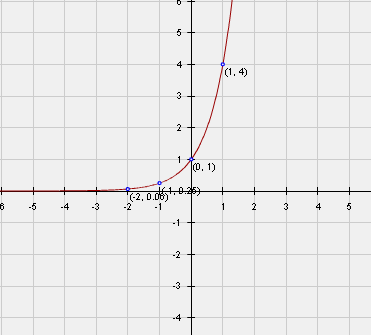
\includegraphics[scale=0.4]{graph9}\\ (1) Determine an equation of the form $y=Cb^x$ for the above graph.} {Card 4: $f(x)=4^x$}

\card{A piece of machinery, initially purchased for \$25,000, decreases in value by 1.4\% per year. Determine a model of the form $v=k \cdot b^t$ that can be used to predict the value of this machinery if t is measured in years.}{Card 5: $v=25000 \cdot (0.986)^t$}

\card{How much money should you invest at 7.5\% compounded quarterly so that you have \$10,000 after 5 years?}{Card 6: \$6896.80}

\card{Solve for $x$: \[\frac{e^{x+5}}{x^{3x}}=e^{x-1}\]}{Card 7: x=2}

\card{Samantha invested \$300 in an investment account that earned 4.6\% interest compounded continuously for 40 years. How much money is in the account after 40 years? }{Card 8: \$1888.96}

\card{A species of snake was introduced in an area 10 years ago. It is estimated that there are 3500 snakes in the area now, and the population has a relative exponential growth rate of 7\% per year. How many snakes will there be 20 years from now?}{Card 9: 14194}

\card{Write the following as a logarithm:\\ (1) $2^x=3$\\ (2) $245^{\frac{1}{2}}=x$\\ (3) $b^x=y$}{Card 10: (1) $\log_2(3)=x$\\ (2) $\log_{245}x=\frac{1}{2}$\\ (3) $\log_by=x$ }

\card{Write the following as an exponential:\\(1) $\log_2(3)=x$\\ (2) $\log_{245}x=\frac{1}{2}$\\ (3) $\log_by=x$ }{Card 11: (1) $2^x=3$\\ (2) $245^{\frac{1}{2}}=x$\\ (3) $b^x=y$}

\card{Consider the equation: \[f(x)=\log_3(x+11)\] (1) What is the domain of $f(x)$?\\ (2) What is the range of $f(x)$?\\ (3) What is the asymptote of $f(x)?$}{Card 12: (1) $(-11, \infty)$\\ (2) All real numbers\\ (3) $x=-11$}

\card{Determine the inverse of:\\ (1) $f(x)=3^{x-7}+2$\\ (2)$g(x)=\ln(x-4)+3$\\ (3)$h(x)=2\log_5(x+5)-4$ }{Card 13: (1) $\log_3(x-2)+7$\\ (2) $e^{x-3}+4$\\ (3) $5^{\frac{x}{2}}-5$}

\card{Expand:\\(1) $\log_5\left(\frac{ab^2}{5cd}\right)$\\ (2) $\ln\left(\frac{e^2}{3}\right)$\\ (3) $\log_7\left(\frac{7abc}{d^2}\right)$}{Card 14: Hehehe}

\card{Write as a single logarithm:\\ (1) $\log_5(x)+2\log_5(y)-\log_5(z)-1$\\ (2) $\ln(x)+\frac{1}{3}\ln(27)-\ln(y)+\ln(z)$\\ (3) $\log_7(x)-\log_7(3)+4\log_7(y)-1$}{Card 15: Yeah!}

\card{How long would it take to double your investment if you invest \$2,000 at 7.5\% compounded quarterly?}{Card 16: 9.32 years}

\card{Suppose 128 ounces of a radioactive substance exponentially decays to 28 ounces in 6 hours. What is the half-life of the substance?}{Card 17: -25.33\%}

\end{document} 